\chapter{An Incomplete Theory}
\label{sec:theo}

One of the great questions that humans have always tried to answer is
what are the fundamental building blocks of the universe and what are the rules that govern them?
Attempts at answering this question have ranged from the
philosophical approach of \textit{`atomism'} by the ancient Greeks \cite{theo-atomism}
to the discovery of atomic structure by Ernest Rutherford \cite{theo-rutherford}.

The current best answer to this question is the \textit{`Standard Model of Particle Physics'},
a mathematical description of a finite set of fundamental particles and their interactions.
The Standard Model's ability to describe data is formidable
and as such it is the foundation of the field of Particle Physics. 
However, it is known that this is not a complete theory and there must be
a deeper underlying theory that lies beyond the Standard Model.

This chapter firstly aims to describe the Standard Model and its key predictions
with respect to the analyses within the context of this thesis.
Section~\ref{sec:theo-sm} briefly describes the Standard Model and
Section~\ref{sec:theo-qcd} outlines the QCD description of jet formation and dijet production in proton-proton collisions.
Then, Section~\ref{sec:theo-bsm} will discuss Beyond the Standard Model (BSM) physics;
specifically what are the problems in the Standard Model that require BSM physics
and what evidence of BSM physics could be found at the ATLAS collider.

\newpage
\section{The Standard Model}
\label{sec:theo-sm}

The Standard Model is a quantum field theory,
meaning that the theory describes a finite set of particles and their interactions in
terms of a set of fields.
The end product of the Standard Model is a prediction
of what will happen when any two particles in nature interact;
which in the context of a collider experiment means predicting what is the cross-section of any given interaction.

Section~\ref{sec:theo-sm_particles} contains a description of the particles that make up the Standard Model 
and Section~\ref{sec:theo-sm_forces} contains a description of the types of interactions between the particles, known as forces.

\subsection{Particles}
\label{sec:theo-sm_particles}

There are 18 fundamental particles in the Standard Model,
where fundamental means that they are not composed of other constituent particles.
These particles are grouped into three families with similar properties;
known as quarks, leptons and bosons.
Details on the particles in the Standard Model is taken from~\cite{obj-bjets_PDG}, where a full description can be found.

\begin{itemize}[leftmargin=*]
\item\textbf{Quarks:}
  Quarks are fermions, meaning they are spin-$\frac{1}{2}$ particles,
  that interact with the strong force; a description of the strong force is in the next section.
  There are 6 different types of quarks, known as flavours, arranged in 3 generations.
  Table~\ref{tab:theo-sm_quarks} summarises the flavours of quark and their key properties.
  For each quark there is also an anti-quark, which has identical mass and spin, but opposite charge and quantum numbers.
  %\end{itemize}
  {\renewcommand{\arraystretch}{1.5}
  \begin{table}[!ht]
  \begin{center}
    \begin{tabular}{|c||c|c|c|c|}
      \hline
    Quark Flavour & Symbol & Charge            &  Spin           &  Mass [GeV]\\
    \hline
    Up            &   $u$  &  $+\frac{2}{3}$   &  $\frac{1}{2}$  &  0.002\\
    Down          &   $d$  &  $-\frac{1}{3}$   &  $\frac{1}{2}$  &  0.005\\
    \hline                                                   
    Charm         &   $c$  &  $+\frac{2}{3}$   &  $\frac{1}{2}$  &  1.3 \\
    Strange       &   $s$  &  $-\frac{1}{3}$   &  $\frac{1}{2}$  &  0.096 \\
    \hline                                                      
    Top           &   $t$  &  $+\frac{2}{3}$   &  $\frac{1}{2}$  &  173  \\
    Bottom        &   $b$  &  $-\frac{1}{3}$   &  $\frac{1}{2}$  &  4.2  \\
    \hline  
  \end{tabular}
    \caption{The key properties of the 6 flavours of quark in the Standard Model,
    organised into the three generations of quarks.}
  \label{tab:theo-sm_quarks}
  \end{center}
  \end{table}}

\item\textbf{Leptons:}
  Leptons are fermions that, unlike the quarks, do not interact with the strong force.
  There are 6 different types of leptons,
  arranged into  3 generations, each containing a charge $-1$ particle and a charge 0 neutrino.
  Table~\ref{tab:theo-sm_leptons} summarises the leptons and their key properties.
  Neutrinos masses are not well known, but they are known to be non-zero
  and the sum of the masses of the three flavours of neutrino is less than a few eV~\cite{theo-nu_mass}
  \footnote{The upper constraint on neutrino mass means that neutrinos are much lighter than the other particles
  in the Standard Model and the energy scale considered in this thesis; so they will be treated as massless here.}
  For each lepton there is also an anti-lepton.
  
  {\renewcommand{\arraystretch}{1.5}
  \begin{table}[!ht]
  \begin{center}
    \begin{tabular}{|c||c|c|c|c|}
      \hline
    Lepton            & Symbol        & Charge  &  Spin           &  Mass [GeV]\\
    \hline
    Electron          &   $e$         &  -1    &  $\frac{1}{2}$   &  \num{5.1e-4}\\
    Electron Neutrino &   $\nu_e$     &  0     &  $\frac{1}{2}$   &  -\\
    \hline                                   
    Muon              &   $\mu$       &  -1    &  $\frac{1}{2}$   &  0.11 \\
    Muon Neutrino     &   $\nu_{\mu}$  &  0     &  $\frac{1}{2}$   &  -\\
    \hline                                      
    Tau               &   $\tau$       &  -1   &  $\frac{1}{2}$   &  1.8\\
    Tau Neutrino      &   $\nu_{\tau}$  &  0    &  $\frac{1}{2}$   &  -\\
    \hline  
  \end{tabular}
    \caption{The 6 types of lepton in the Standard Model and their key properties,
    organised into the three generations of leptons. Neutrino masses are not well known. }
  \label{tab:theo-sm_leptons}
  \end{center}
  \end{table}}
 
\item\textbf{Bosons:}
  There are a set of integer-spin particles in the Standard Model, known as bosons.
  The bosons of the Standard Model act as the mediators of the forces that will be described below.
  Table~\ref{tab:theo-sm_bosons} summarises the bosons and their key properties.
  %The bosons are their own anti-particle, with the exception of the $W^{+}$ and $W^{-}$
  %which are each others anti-particle.

  {\renewcommand{\arraystretch}{1.5}
  \begin{table}[!ht]
  \begin{center}
    \begin{tabular}{|c||c|c|c|c|}
      \hline
    Boson            & Symbol        & Charge  &  Spin  &  Mass [GeV]\\
    \hline
    Photon           &   $\gamma$    &  0      &  1     &  0 \\
    W-boson          &   $W^{\pm}$    & $\pm$1  &  1     &  80 \\
    Z-boson          &   $Z_0$       &  0      &  1     &  91\\
    Gluon            &   $g$         &  0      &  1     &  0 \\
    Higgs Boson      &   $H$         &  0      &  0     &  125\\
    \hline  
  \end{tabular}
    \caption{The key properties of the bosons of the Standard Model. }
  \label{tab:theo-sm_bosons}
  \end{center}
  \end{table}}
    
\end{itemize}

\subsection{Forces}
\label{sec:theo-sm_forces}

The Standard Model combines three key theories in a
$SU(3)~\text{x}~SU(2)~\text{x}~U(1)$ gauge symmetry.
The first key theory is the electro-weak theory~\cite{theo-glashow};
this theory is based on mixing within the symmetry group $SU(2)~\text{x}~U(1)$
leading to three distinct interaction types grouped into two forces:
the electro-magnetic and weak forces.
The second is Quantum Chromodynamics (QCD)~\cite{theo-qcd} which describes the strong force.
Finally, the Brout-Englert-Higgs Mechanism~\cite{theo-be,theo-higgs} describes the origin of mass in the Standard Model.

\noindent
Each interaction is discussed in greater detail below:
\begin{itemize}[leftmargin=*]
\item\textbf{Electro-magnetic (EM):}

  The EM force is an interaction between charged particles and is mediated by the photon.
  The strength of a force is often given in terms of the coupling constant, $\alpha$.
  In this case the EM coupling is proportional to the EM coupling constant, $\alpha_{EM}$,
  multiplied by the product of the charges of the two particles, where $\alpha_{EM} \sim$ 1/137.\\ %\vspace{0.5em}

\item\textbf{Weak Force:}
  
  The weak force is composed of the two remaining interactions from electro-weak theory;
  the neutral current interaction and the charged current interaction.
  
  The neutral current interaction is mediated by the $Z_0$ boson, has a universal interaction to all fermions,
  and does not allow for flavour change within the interactions.

  The charged current interaction is mediated by the $W^+$ and $W^-$ boson, has a universal interaction with all fermions,
  and flavour changing interactions are allowed.
  In the quark sector, the fact that the charged current interaction couples with weak eigenstates of fermions rather than
  their flavour eigenstates,
  the charged current interaction allows for interactions that change generation of the quark's flavour.
  The relative amplitudes of each flavour changing interactions is described by the CKM matrix;
  the structure of this matrix suppresses generational changing interactions,
  in particular those from the 3rd generation  are highly suppressed.
  This feature will prove important for identifying the presence of $b$-quarks at the ATLAS detector.
  Both interactions of the weak force are much weaker than the EM force due to the large masses of the mediating particles
  ($\text{Weak}/\text{EM} \sim 10^{-4}$).\\ %\vspace{0.5em}
  
\item\textbf{Strong Force:}

  Quantum Chromodynamics (QCD) is a theory described by a SU(3) gauge symmetry that describes the interactions between quarks and gluons.
  The symmetry leads to 3 colour charges: known as red, green and blue.
  An anti-quark has colour charge anti-red, anti-blue or anti-green.
  A colour neutral object can be formed if all three colour charges are present (i.e. in a Baryon containing three quarks)
  or if a colour and the corrosponding anti-colour is present (i.e. in a Meson that contains $q\bar{q}$).
  The strong force is mediated by the gluon and interacts with particles that have colour charge; which are quarks and gluons.
  The fact that the gluon has colour charge means that the gluon is self interacting.
  QCD is important in terms of understanding hadronic jet formation and the production of the
  largest background in a dijet search, so further details can be found in section in Section~\ref{sec:theo-qcd}.\\

\item\textbf{Higgs Mechanism:}
  The Higgs Mechanism \footnote{Also known as the Higgs-Englert-Brout mechanism}
  introduces an extra scalar field to the Standard Model
  with a Higgs potential given by the so-called `Mexican-hat potential'.
  This allows for spontaneous symmetry breaking which gives mass to the bosons of the Standard Model.
  In addition, a Yukawa coupling term between the scalar field and the fermions gives rise to the mass of the fermions
  \footnote{With the exception of the neutrinos, whose mass is not described by the Standard Model}.
  A final prediction of the Higgs mechanism is the existence of a spin-0 boson, known as the Higgs boson.
  The first observation of the Higgs Boson like object by the ATLAS~\cite{theo-higgs_atlas} and CMS~\cite{theo-higgs_cms} experiments
  in 2012 appears to confirm the Higgs mechanism, which is seen as a great triumph of the Standard Model.
\end{itemize}

\section{QCD: Hadronic Jet Formation and Dijet Production}
\label{sec:theo-qcd}

As described above Quantum Chromodynamics (QCD) is a theory that describes the strong interaction between
quarks and gluons.
QCD therefore describes two elements that are critical to the analysis being presented in this thesis;
specifically the formation of hadronic jets and the production of dijet events through QCD in proton-proton collisions,
which will be the dominant background in the analysis presented in this thesis.

This section will firstly describe renormalisation of QCD, which is important for understanding how QCD works,
and will then describe the process of hadronic jet formation and dijet production in hadron collisions.
Quarks and gluons can often fill similar roles in hadronic jet formation and dijet production, hence I will refer to them collectively as `partons' in this section.

\subsection{Renormalisation and the Running of $\alpha_S$}
\label{sec:theo-qcd_dijet_running}

For any calculation in QCD, or indeed any quantum field theory, one must consider the higher order loop diagrams;
for example for a simple gluon propagator there are additional first-order loops as shown in Figure~\ref{fig:theo-qcd_gluon}.
These additional loops lead to divergences in calculations of scattering events in QCD.

\begin{figure}[!hbt]
  \begin{center}
    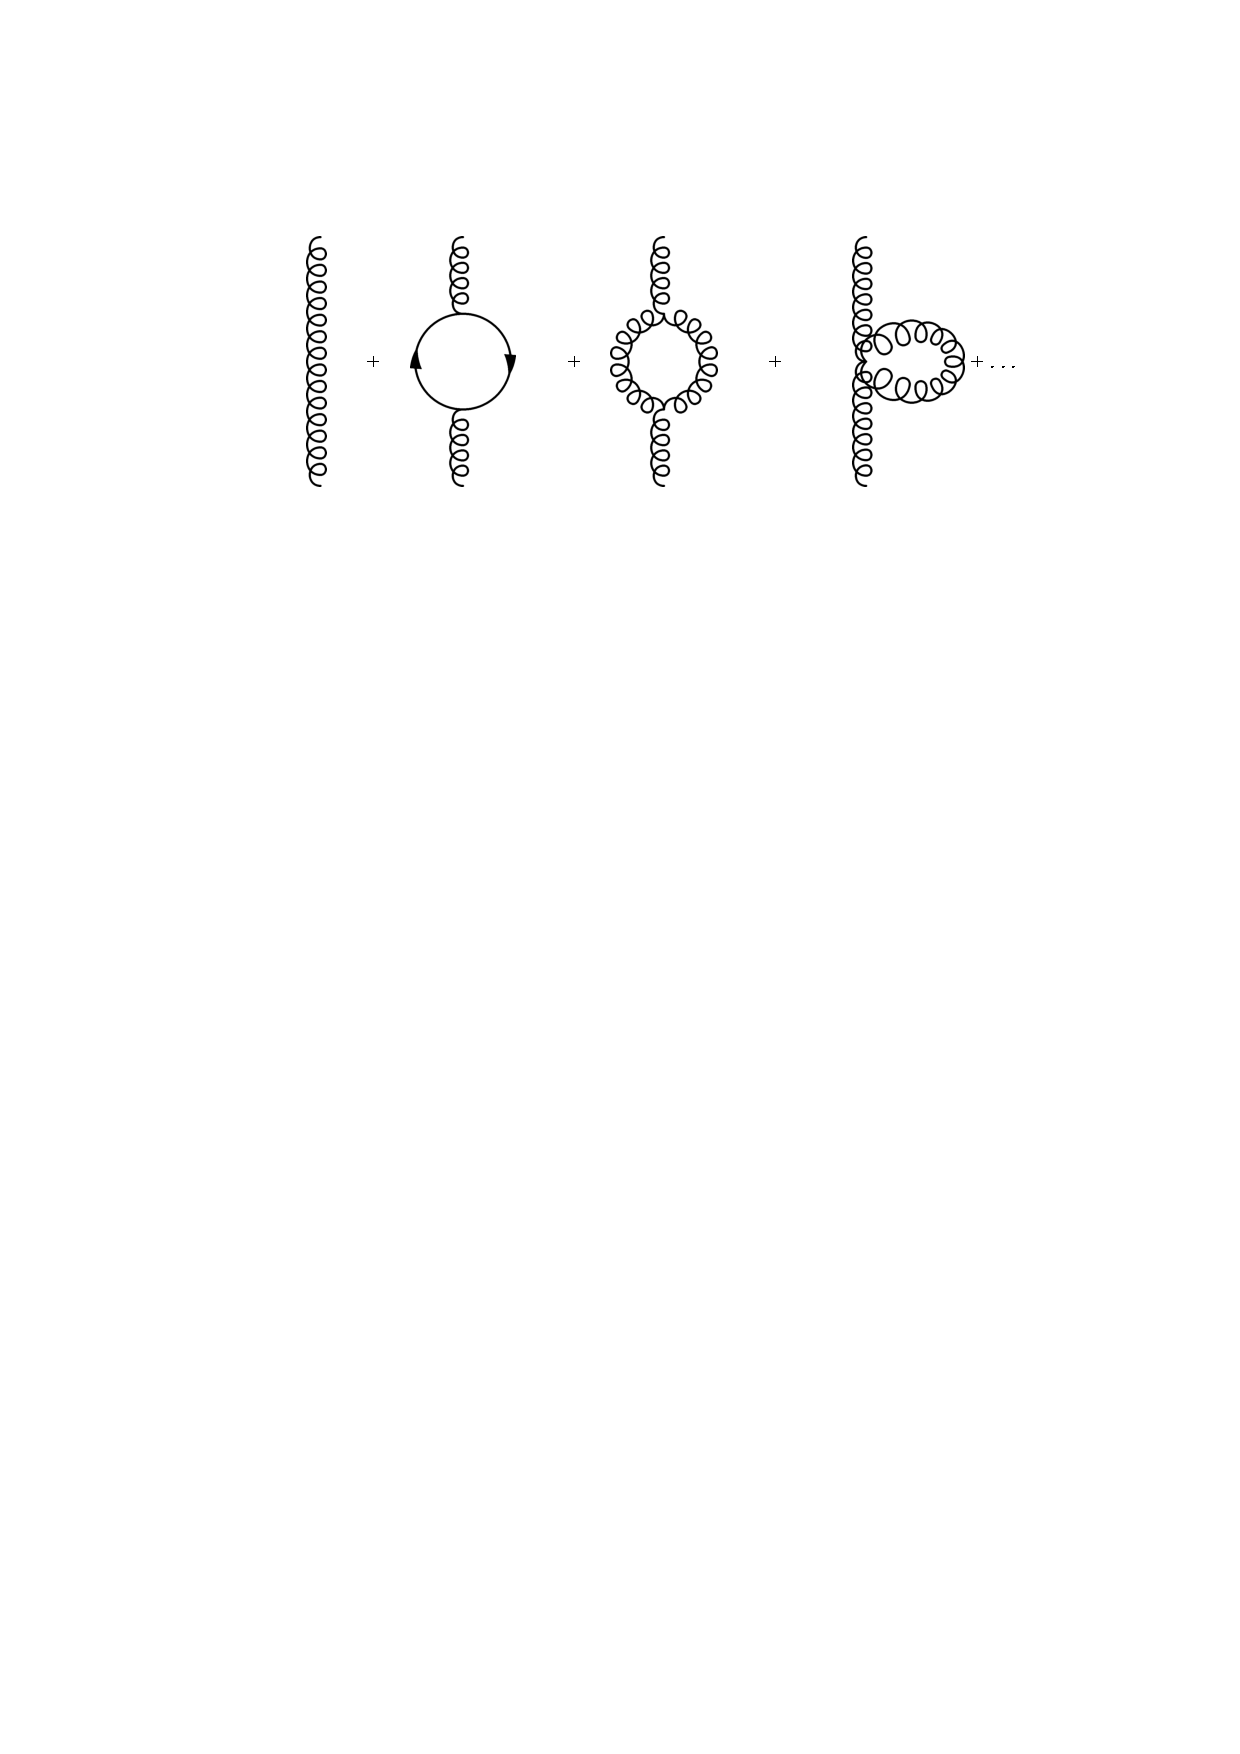
\includegraphics[width=0.7\linewidth, angle=0]{figs/Theory/qcd_gluon_loop.pdf}
  \end{center}
  \caption[A schematic showing the gluon propagator with the additional first order loops.]
  {A schematic showing the gluon propagator with the additional first order loops~\cite{det-thesis_kate}.}
  \label{fig:theo-qcd_gluon}
\end{figure}

To avoid these divergences, there is a well accepted mathematical tool known as renormalisation,
where one effectively re-scales the fields in the Lagrangian.
This is done such that the divergences are removed
and one can perform calculations of QCD in a perturbative expansion.
This leads to a dependence of the strong coupling, $\alpha_S$, on the renormalisation scaled used, $\mu_R$,
an effect known as the running of $\alpha_S$.
To get a an effective strength of the strong interaction in any given process,
once sets the value of $\mu_R$ to be the scale of the momentum transfer $Q$ of the process.
%%which is the natural choice for the process.
%$\alpha_S($\mu_R \sim Q^{2}$).
The running of $\alpha_S$ can be measured through experimental observation;
Figure~\ref{fig:theo-qcd_running} shows the measured values of
the strong coupling constant, $\alpha_S$ as a function of the energy scale, $Q$, in a range of experiments.

\begin{figure}[!hbt]
  \begin{center}
    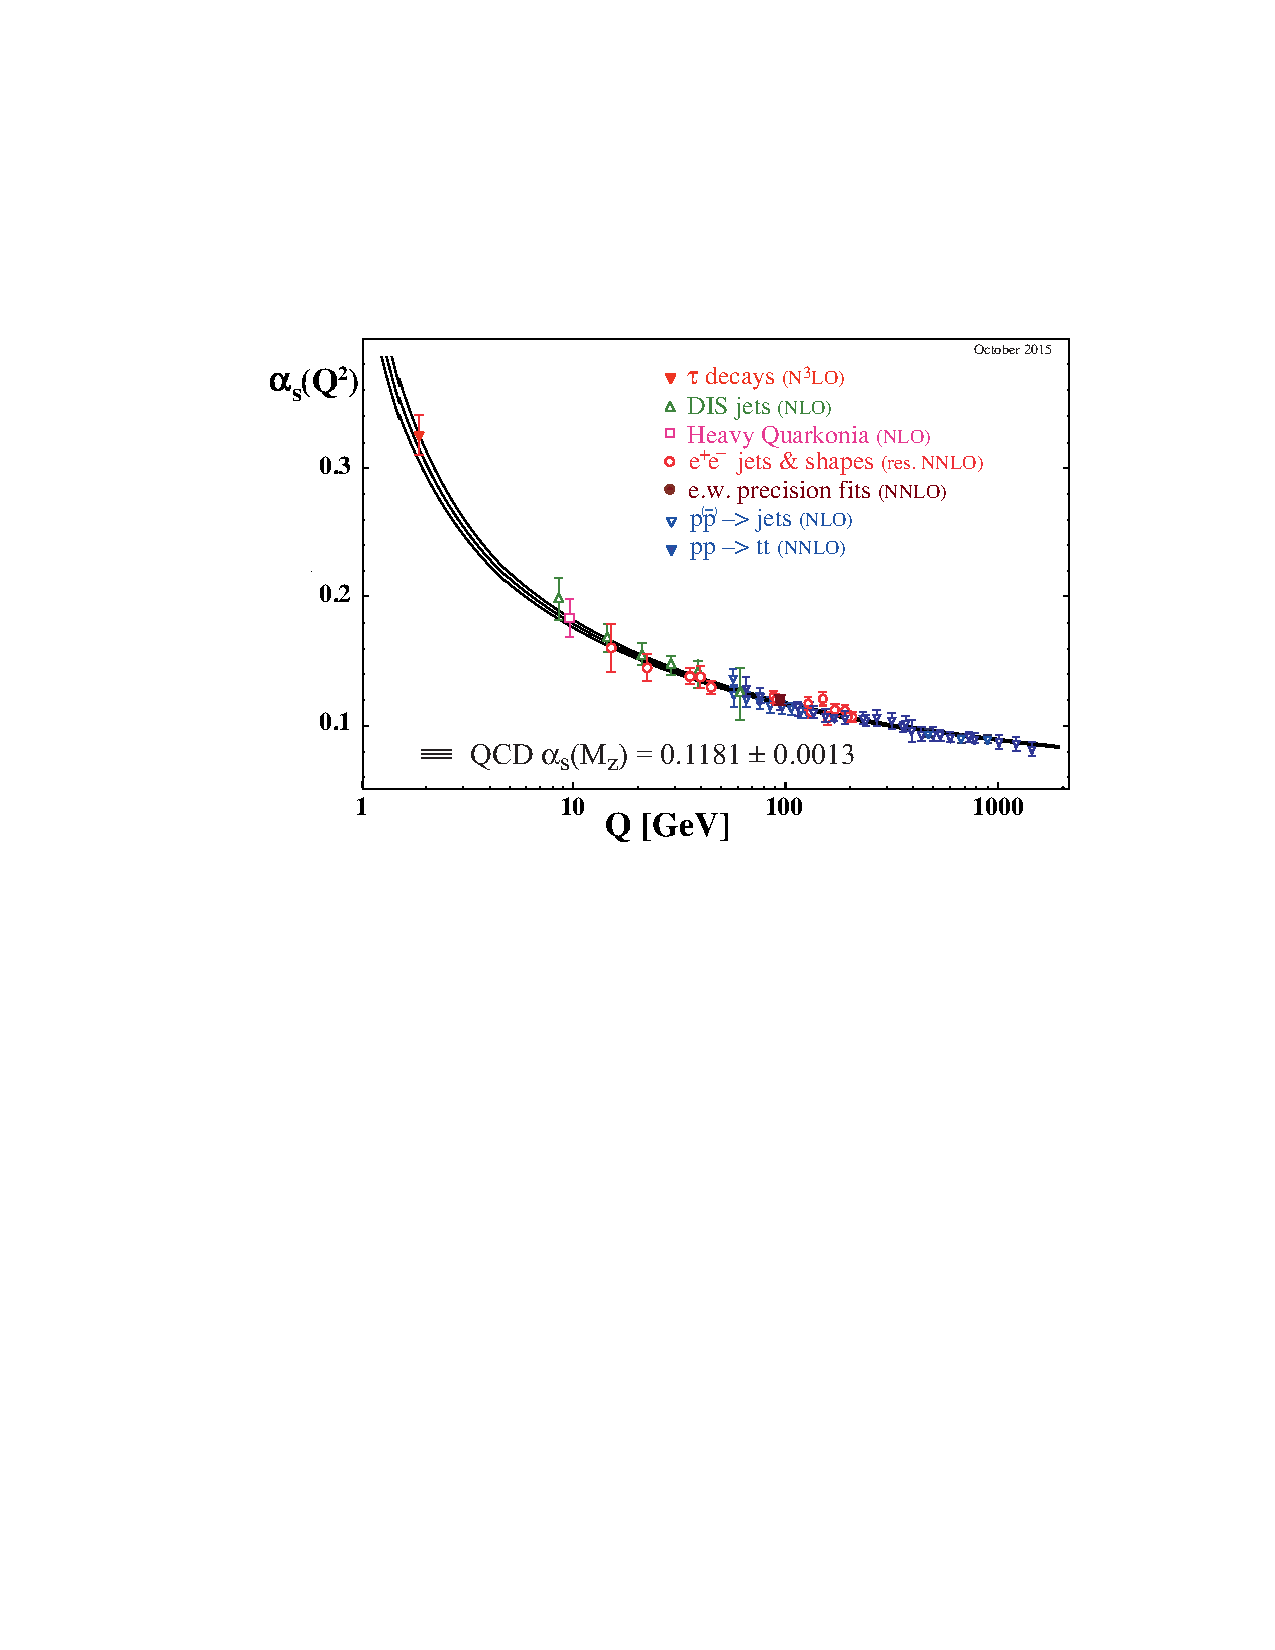
\includegraphics[width=0.7\linewidth, angle=0]{figs/Theory/qcd_running.pdf}
  \end{center}
  \caption[Summary of measurements of $\alpha_S$ as a function of the energy scale $Q$.
    The respective degree of QCD perturbation theory used in the extraction of $\alpha_S$ is indicated in brackets
    (NLO: next-to-leading order; NNLO: next-to-next-to leading order; res. NNLO: NNLO matched with resummed next-to-leading logs; N3LO: next-to-NNLO).]
          {Summary of measurements of $\alpha_S$ as a function of the energy scale $Q$.
            The respective degree of QCD perturbation theory used in the extraction of $\alpha_S$ is indicated in brackets
            (NLO: next-to-leading order; NNLO: next-to-next-to leading order; res. NNLO: NNLO matched with resummed next-to-leading logs; N3LO: next-to-NNLO)~\cite{theo-qcd}.}
  \label{fig:theo-qcd_running}
\end{figure}

There are three features of Figure~\ref{fig:theo-qcd_running} that can be noted.
Firstly that the size of the coupling constant, $\alpha_S$, is generally large compared to the $\alpha_{EM} \sim 1/137$;
this means that, depending on the energy scale $Q$, the strong force is typically stronger than the $EM$ force by one or two orders of magnitude.
Secondly, at high-energies/low-distance scales the strong force becomes realtively weak, this phenomenon is known as
\textit{`asymptotic freedom'}.
At these energy scales, perturbative expansions of QCD are possible.
Finally, at low-energies/large-distance scales the strong force is exceptionally strong.
As a result, if two interacting quarks become separated by a large distance then it becomes energetically favourable to
pair-produce a $q\bar{q}$ pairs from the vacuum until a colour neutral object can be formed.
Therefore quarks will never be observed in isolation but instead quarks form colour neutral hadrons, this feature of QCD is known as \textit{`confinement'}.

\subsection{Hadronic Jet Formation}
\label{sec:theo-qcd_jets}

It is common in hadronic colliders that a high-momentum quark or gluon will be produced in the final-state,
an example of this is dijet production, as described in Section~\ref{sec:theo-qcd_dijet}.
However, as described in Section~\ref{sec:theo-qcd_dijet_running},
the large values of $\alpha_S$ at large distance-scales require quark confinement, meaning that an isolated quark or gluon will not be observed.
Instead a stream of energetic, collimated hadrons will be formed, known as a hadronic jet.
Hadronic jet formation is described by two distinct processes; parton-shower and hadronisation.

\begin{itemize}[leftmargin=*]
  
\item\textbf{Parton Shower:}

  The high-energy final-state quark or gluon has a finite probability of splitting into a quark-gluon or quark-quark pair respectively.
  The resulting quarks and gluons will also undergo splitting to form more partons,
  which in turn can split. This process continues to form the parton shower.
  Due to relativistic effects, each splitting will generally be at a small opening angle in the lab-frame
  and as such the partons will be highly collimated in the direction of the initial parton.
  The parton shower process occurs at high energy such that the value of $\alpha_S$ is small
  and thus perturbative expansions of QCD can be used to perform calculations.
  However, at each step of the splitting the energy of the partons decreases
  and thus the value of $\alpha_S$ increases.\\
  
\item\textbf{Hadronisation:}
  
  When the energy scale becomes small
  \footnote{This is generally defined as small relative to the hadronic scale, $\Lambda$, which is typically a few hundred MeV},
  $\alpha_S$ becomes large such that the dominant QCD effect is quark confinement.
  Therefore, $q\bar{q}$ pairs are produced until the quarks resulting from the parton shower can form hadrons.
  The hadrons are colour neutral objects, meaning that stable hadrons that do not interact through QCD will be formed
  \footnote{Some unstable hadrons, such as a $\Delta^{++}$, may be initially formed in the process but these will decay rapidly through the strong interaction.
    In addition, some hadrons might not be stable under the weak interaction, such as a Kaon, but the time-scale of their decays will be much larger.}.
  The hadronisation process occurs at large values of $\alpha_S$ so cannot be calculated using perturbative expansions;
  to simulate hadronisation models such as the string model~\cite{theo-qcd_jet_string} and the
  cluster model~\cite{theo-qcd_jet_cluster} are used.

\end{itemize}
  
The end result of the hadronisation process is a set of collimated stable hadrons,
known as a hadronic jet, which can be observed in an experiment.
Note that our understanding of how one goes from an initial parton to a hadronic jet is model dependant,
for example there is a choice of hadronisation model.
Hence, in experiment we remove this dependence by defining a jet in terms of observables,
such that the experimental results are model-independent and results can be reinterpreted when improved models become available
\footnote{A good explanation of why model-independent jets is desirable is found here~\cite{theo-jets_jb}}.
The details of the experimental definition of a hadronic jet is discussed in Section~\ref{sec:obj-jets}.

%\subsection{Parton shower}
%\subsection{Hadronisation}

\subsection{Dijet Production in $pp$ Collisions}
\label{sec:theo-qcd_dijet}


Dijet production is one of the most common process that occurs in any hadron collider.
The first step of dijet production in $pp$ colliders is the two protons interacting through QCD to give two quarks or gluons in the final state;
the frequency of this interaction is described by the hadronic cross-section, $\sigma_{had}$.
The free partons will then form hadronic jets through the processes described in Section~\ref{sec:theo-qcd_jets}, which can be observed.
As an example, Figure~\ref{fig:theo-qcd_dijet_feynman} shows the Feynman diagram of
dijet production in a proton-proton collision through the qg$\to$qg channel.

\begin{figure}[!hbt]
  \begin{center}
    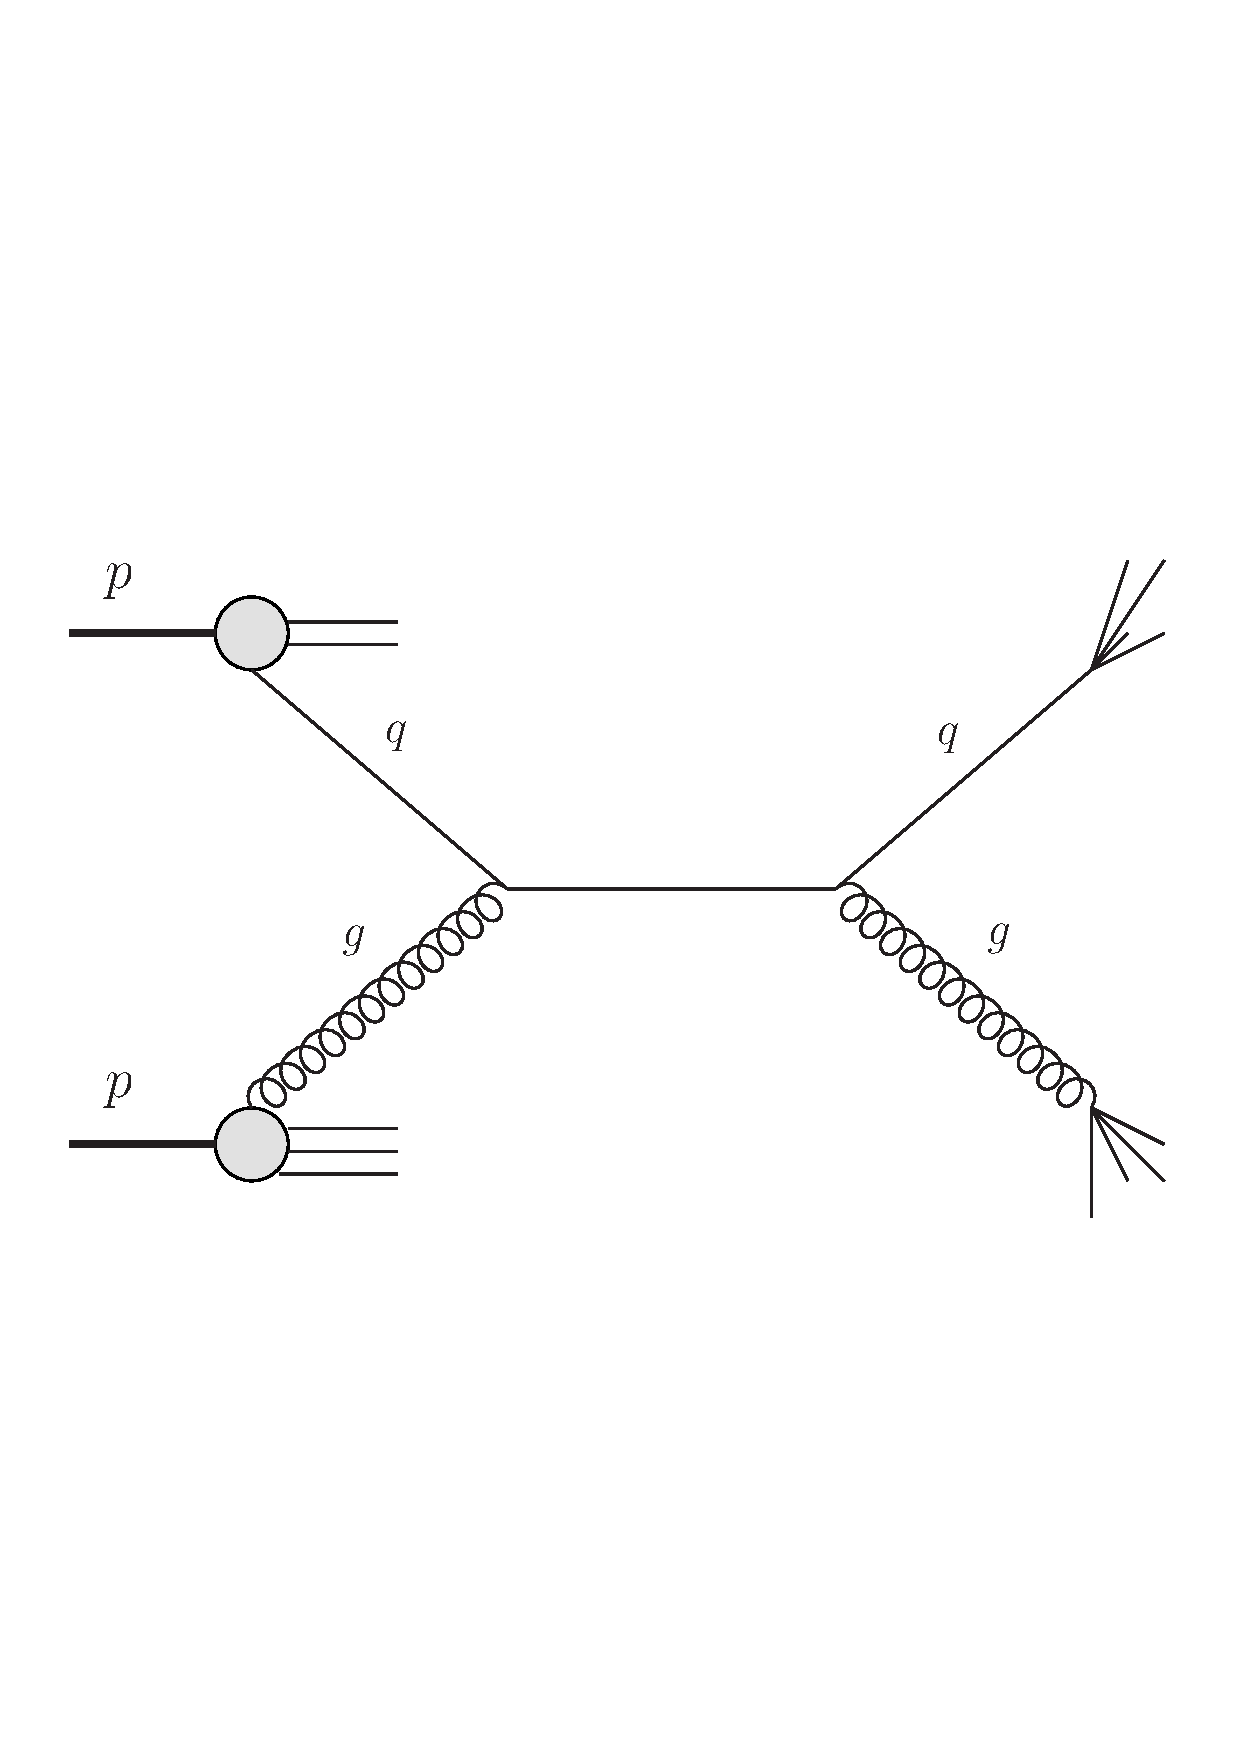
\includegraphics[width=0.7\linewidth, angle=0]{figs/Theory/qcd_dijet_feynman.pdf}
  \end{center}
%  \caption[Three feynman diagrams illustrating the parton level scatter process in dijet production at the LHC.]
%          {Three feynman diagrams illustrating the parton level scatter process in dijet production at the LHC~\cite{theo-qcd_dijet_feynman}.}
  \caption[A Feynman diagram showing dijet production in a proton-proton collision through the qg$\to$qg channel.]
          {A Feynman diagram showing dijet production in a proton-proton collision through the qg$\to$qg channel. Adapted from~\cite{theo-qcd_dijet_feynman}.}
  \label{fig:theo-qcd_dijet_feynman}
\end{figure}

\subsubsection{Factorisation}

To calculate the hadronic cross-section, $\sigma_{had}$, in a proton-proton collision,
two elements are separated out in a process called factorisation.

The first element is the parton-level cross-section, $\hat{\sigma}$, which is the cross-section of
two partons from the proton ($p_a$ and $p_b$) scattering to give two final state partons ($p_i$ and $p_j$).
This is effectively the central part of the Feynman diagram in Figure~\ref{fig:theo-qcd_dijet_feynman}.

The second element is the Parton Density Functions (PDFs), $f_a(x_a)$, which describes the number density of
a specific parton, $p_a$, with momentum fraction, $x_a$, in a proton.
Momentum fraction is defined as the fraction of the protons total momentum that the parton is carrying, $x = p_{\text{parton}}/p_{\text{proton}}$.
The number density affects the overall cross-section, as it changes the probability that a specific parton
can form the inital parton propagators.
This part of the interaction is indicated by the circles in the
top and bottom left of the Feynman diagram in Figure~\ref{fig:theo-qcd_dijet_feynman}.

The elements are combined to calculate the total $\sigma_{had}$;
\begin{equation}
%  \sigma(p_1p_2\to q/g_i q/g_j) = \int dx_1 dx_2 f_1(x_1,\mu^2_F)f_2(x_2\mu^2_F) \sigma(q/g_1,q/g_2, \alpha_s(\mu^2_R),Q^2/\mu^2_F,Q^2/\mu^2_R)
  \sigma_{had} = \sum_{a,b,i,j} \int dx_a dx_b f_a(x_a,Q^2)f_b(x_b,Q^2) \hat{\sigma}(p_a, p_b\to p_i p_j)
\end{equation}
where there is an integral over all possible values of momentum fractions $x_a$ and $x_b$,
a sum over all possible partons from the two protons labelled $a$ and $b$,
and a sum over all possible final-state partons labelled by $i$ and $j$.
$Q^2$ is the energy scale of the collision.

With the two elements separated we can discuss each separately.

\subsubsection{Parton-level Cross-Section}
\label{sec:theo-qcd_dijet_xs}

To describe the parton-level cross-section we must first define a few variables.
The first is the invariant mass of the outgoing partons, $m_{ij}$, which is given in terms of the four-momentum of the two partons by;
\begin{equation}
  m_{ij}^2 = (p^\mu_i + p^\mu_j)^2  
\end{equation}
\noindent
Then there are two related angular variables, $y^*$ and $\theta^*$,
defined in terms of $y_i$, the rapidity of the outgoing parton $p_i$;
\begin{equation}
  y^* = (\frac{y_i - y_j}{2}),
\end{equation}
\begin{equation}
  cos(\theta^*) = \tanh(y^*)
\end{equation}
\noindent
Finally the Mandelstam variables, generally used to describe a 2$\to$2 particle scatter event, are defined as 
\begin{equation}
  \hat{s} = m_{ij}^2, \hspace{3mm}  \hat{t} = -\hat{s}\hspace{1mm}(1 - \cos{\theta^*}), \hspace{3mm} \hat{u} = - \hat{s}\hspace{1mm}(1+\cos{\theta^*})
\end{equation}

\noindent
The parton-level cross-section of incoming partons $a$ and $b$ scattering to give
outgoing partons $i$ and $j$ is given in terms of the variables $\theta^*$ and $m_{ij}$~\cite{theo-dijet_harris};
\begin{equation}
  \frac{d\hat{\sigma}(p_a, p_b \to p_i p_j)}{dm_{ij}\hspace{1mm}d\cos{\theta^*}} = \frac{ \pi \alpha_s}{m_{ij}}\hspace{1mm} \text{S}(ab \to ij) \hspace{1mm} \frac{1}{1+\delta_{ij}}
  \label{eq:theo-qcd_dijet_xs}
\end{equation}
Where $\text{S}(ab \to ij)$ gives the process dependant kinematics of a $ab \to ij$  parton scatter.
$\text{S}(ab \to ij)$ for each process is described in Table~\ref{tab:theo-qcd_dijet_s}.

%  {\renewcommand{\arraystretch}{1.5}
%  \begin{table}[!ht]
%  \begin{center}
%    \begin{tabular}{|c|c|}
%      \hline
%      Subprocess         & $\text{S}(ab \to ij)$ \\
%    q1q2 - q1q2          &    4 s + u / 9t       \\
%    q1barq2 - q1barq2    &    4 s + u / 9t       \\
%    q1q1 - q1q1          &    4 s + u / 9t +  4 s + t / 9u
%    q1barq1 - q2barq2
%    
%    \hline  
%  \end{tabular}
%    \caption{The key properties of the 6 flavours of quark in the Standard Model,
%    organised into the three generations of quarks.}
%  \label{tab:theo-sm_quarks}
%  \end{center}
%  \end{table}}
%

\begin{table}[!hbt]
  \begin{center}
    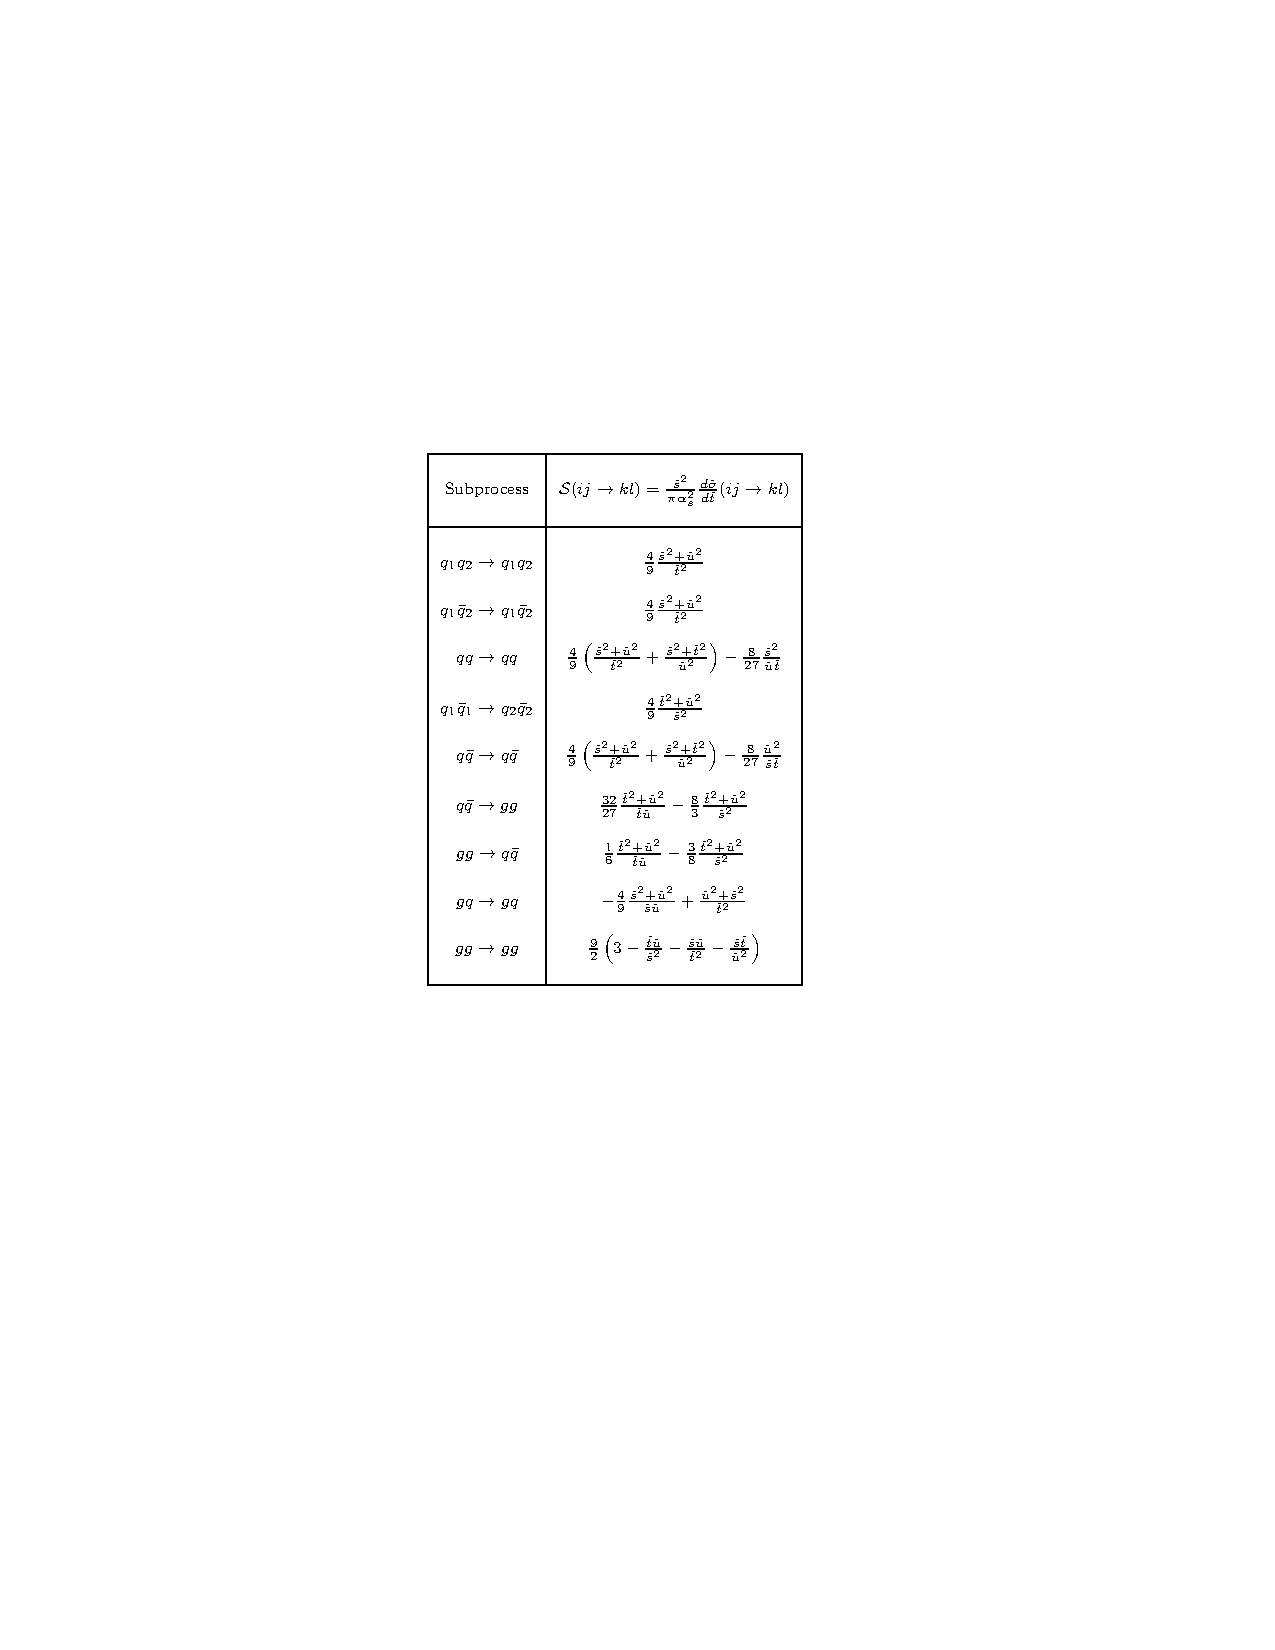
\includegraphics[width=0.7\linewidth, angle=0]{figs/Theory/qcd_dijet_stable.pdf}
  \end{center}
  \caption[A table showing the process dependant part of the parton cross-section, $\text{S}(ab \to ij)$, for each of the processes in dijet production.]
  {A table showing the process dependant part of the parton cross-section, $\text{S}(ab \to ij)$, for each of the processes in dijet production. Taken from Table 1 of~\cite{theo-dijet_harris}.}
  \label{tab:theo-qcd_dijet_s}
\end{table}

\newpage
\subsubsection{Parton Density Functions}
\label{sec:theo-qcd_pdf}

A naive model of the proton contains two up-quarks and a down-quark,
known as valence quarks, each carrying $\frac{1}{3}$ of the proton's momentum.
However, QCD interactions within the proton mean that a gluons can be emmited from the valence quarks
and $q\bar{q}$ pairs can be produced.
Ths means that in reality the proton is made up of the three valence quarks, typically carrying a large fraction of the proton's momentum,
in addition to a sea of quarks and gluons from higher-order QCD effects, that will typically carry a lower fraction of the proton's momentum.

Parton Density Functions (PDFs) give the number density of a specific parton $p_a$ in a proton $P_a$
for a given momentum fraction $x_a$ and energy scale, $Q$.
As QCD is not pertubative in the proton due to the large $\alpha_S$ the PDFs cannot be calculated directly.
Instead the PDFs can be measured by combining a range of experimental scattering results.
In particular, strong constraints on the PDFs come from deep inelastic scattering using $ep$ colliders, such as HERA~\cite{theo-qcd_hera};
the strong constraints are due, in part, to there only being one parton in the collision allowing direct access to the PDFs in a cross-section measurement.

%%%%%%%%%  Note Laurie %%%%%%%%%
%%%% In general one would do e- + p -> e- + jet at HERA
%%%% For sensitiviy to certain versions would could vary the analysis
%%%% For example  e- + s -> mu_e + c->D meson -> mu_e + (jet with muon).

Figure~\ref{fig:theo-qcd_pdf} shows the $x\hspace{0.3mm}F(x,Q^2)$ for a $Q^2$ of 10 and $10^4$ $\text{GeV}^2$
from the MMHT2014 PDF set~\cite{theo-qcd_pdf}.
The various colours lines represent the PDF for each of the different partons.

\begin{table}[!hbt]
  \begin{center}
    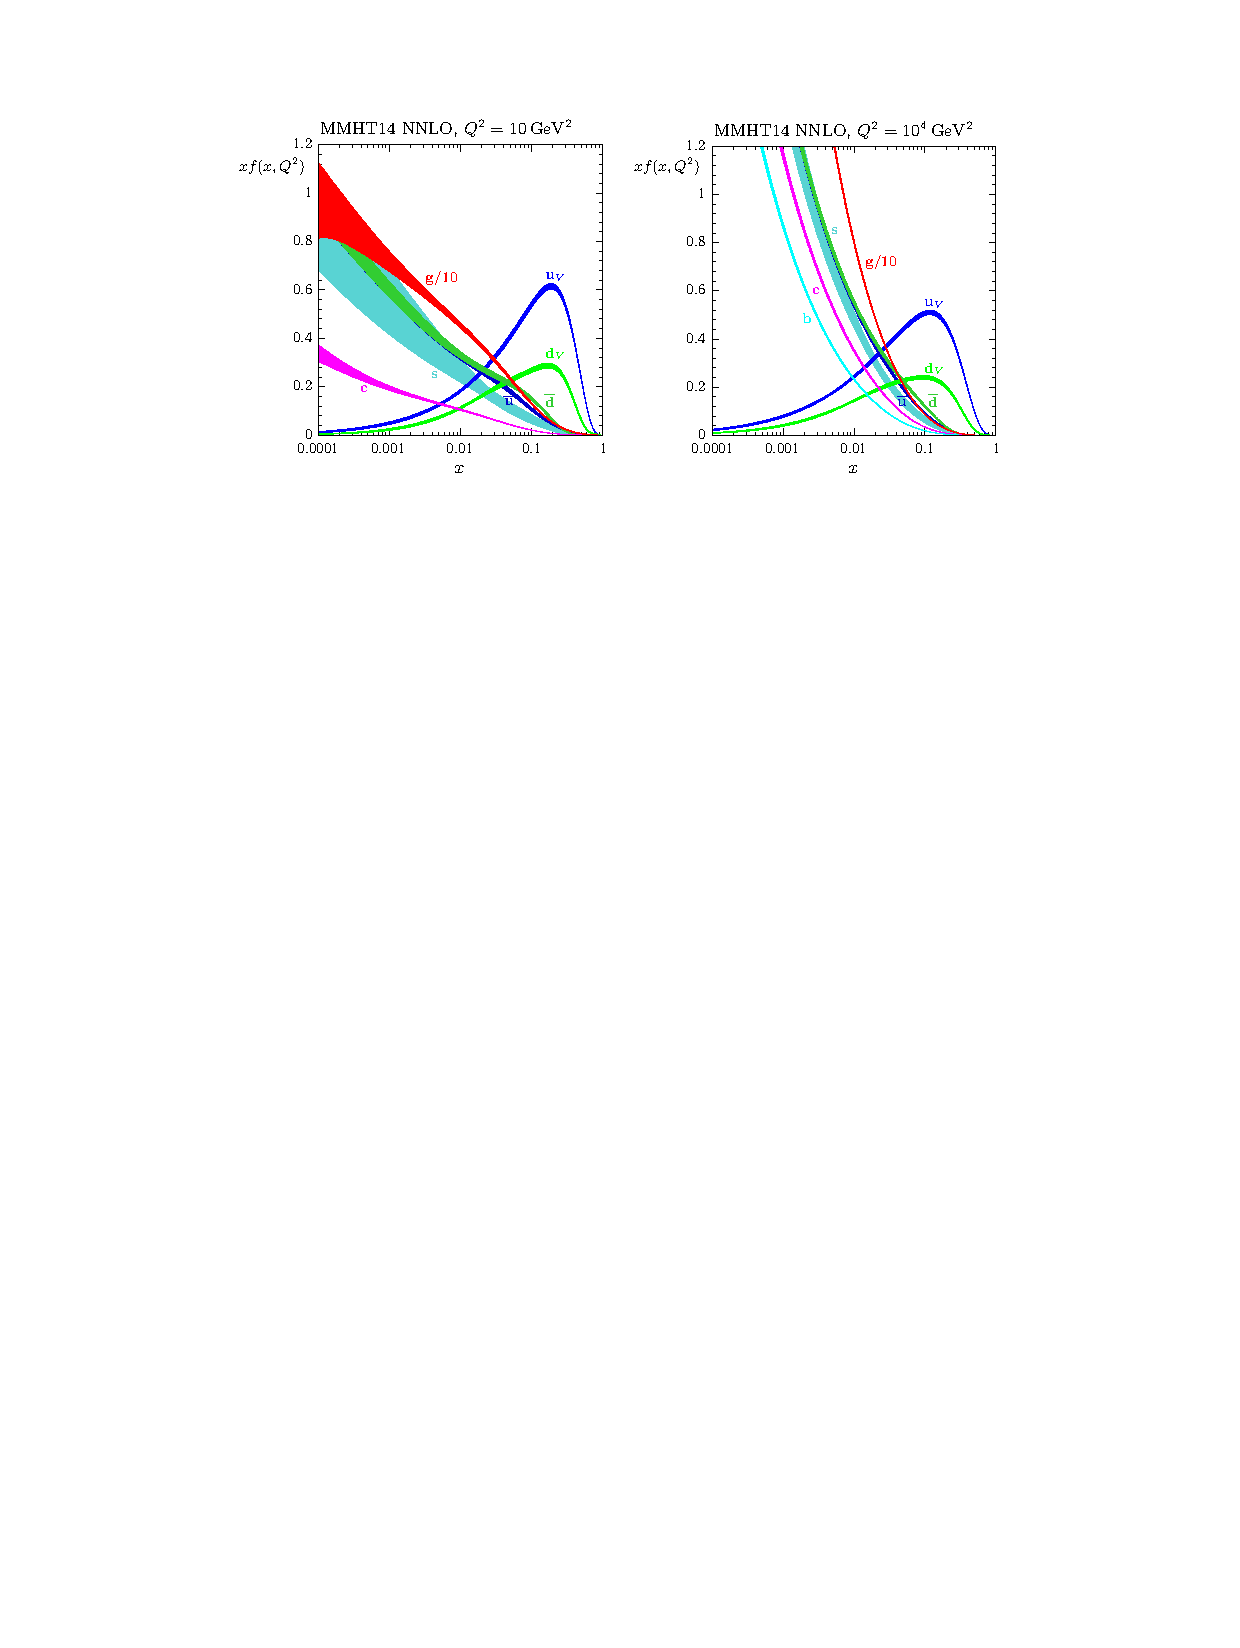
\includegraphics[width=1\linewidth, angle=0]{figs/Theory/qcd_pdf.pdf}
  \end{center}
  \caption[MMHT2014 NNLO PDFs at $Q^2$ = 10 $\text{GeV}^2$ and $Q^2$ = $10^4$ $\text{GeV}^2$, with associated 68\% confidence-level uncertainty bands.]
  {MMHT2014 NNLO PDFs at $Q^2$ = 10 $\text{GeV}^2$ and $Q^2$ = $10^4$ $\text{GeV}^2$, with associated 68\% confidence-level uncertainty bands~\cite{theo-qcd_pdf}.}
  \label{fig:theo-qcd_pdf}
\end{table}

One can note that as $x$ increases the values of the PDF for the sea quarks and gluons will fall smoothly;
this is because it is energetically unfavourable to emmit a high momentum gluon or $q\bar{q}$ pair.
The fall in the PDFs with respect to $x$ is particularly notable for the gluon which is the dominant contribution at low values of $x$.

The PDFs of the valence quarks, $u_v$ and $d_v$, have a peak value around $x \sim \frac{1}{3}$, and then fall off rapidly at higher $x$.
If one considered the proton in the initial naive model of the proton then we find the PDFs of valence quarks as delta peaks at exactly $\frac{1}{3}$
with amplitude of $\frac{2}{3}$ and $\frac{1}{3}$ for the $u$ and $d$ quark respectively;
however, the higher-order QCD effects (which are non-pertubative) have smeared this peak to what is observed.

\subsubsection{Features of the Hadronic Cross-section}

There are three important features that one can qualitatively describe about the dijet hadronic cross-section
from the two factorised elements shown in Section~\ref{sec:theo-qcd_dijet_xs}~and~\ref{sec:theo-qcd_pdf}.
These important features will have significance when forming the dijet search analysis strategy in
Chapters~\ref{bkg}\textit{Background estimation chapter} and~\ref{evt}\textit{Event selection chapter}.

\begin{itemize}[leftmargin=*]
\item\textbf{Large cross-section :}\\
  The strong coupling constant $\alpha_s$ is much larger than the other forces,
  meaning that the dijet cross-section is large.
  As a result dijet production through QCD is one of the most common events at hadron colliders
  and will be the strongly dominant background in any dijet search.\vspace{0.5em}
  
\item\textbf{Behaviour with respect to $m_{ij}$ :}\\
  It can be seen that the hadronic cross-section causes
  a smooth and monotonically decreasing spectrum
  with respect to $m_{ij}$ as a result of three factors.
  Firstly the cross section has a $1/m_{ij}$ term.
  Secondly, as shown in Section~\ref{sec:theo-qcd_dijet_running},
  $\alpha_S$ will smoothly decrease with increasing $Q$, which in this case is linked to $m_{ij}$.
  Finally, as $m_{ij}$ increases then the momentum fraction of the proton, $x$, required to create
  the dijet event will also increase.
  As shown in Figure~\ref{fig:theo-qcd_pdf}, the parton density functions are generally falling 
  with respect to $x$, which will lead to falling behaviour in the hadronic cross-section.
  \vspace{0.5em}
  
\item\textbf{Behaviour with respect to $y^*$ :}\\
  In all but one of the $\text{S}(ab \to ij)$ terms shown in Table~\ref{tab:theo-qcd_dijet_s},
  we see that, due to the $t$-channel diagram, there is a $1/\hat{t}$ term that will become large when $\cos{\theta^*} \to 1$.
  Hence, we find that there is a larger dijet cross-section at large values of $\cos{\theta^*}$ and $y^*$.
\end{itemize}

Finally it should be noted that the above description of the dijet cross-section is
not a full description; I have only considered the tree-level diagrams where
one needs to consider higher orders of QCD to give a fuller description of dijet production.
Related to that issue is the occurance of initial state and final state radiation, known as ISR and FSR respectively.
ISR is when an additional parton is radiated off the incoming parton where FSR is when an additional parton is radiated off the outgoing parton.
This can lead to additional jets in an event, creating a multi-jet event.

One should also consider the Underlying Event (UE) which effectively comprises of the remnants of the proton not used in the hard-scatter.
The UE will mostly be hadronic activity and as a result can lead to additional jets in the event, again giving us a multi-jet event.

\subsection{A Special Case: $t\bar{t}$}
\label{sec:theo-ttbar}

The top-quark is a special case when discussing the formation of jets from quarks.
This results in the unique topology when top-quark pair poduction occurs, known as $t\bar{t}$ events, which is often exploited by analyses.

There are two theoretically motivated features of the top quark which are distinctive.
Firstly, due to the large suppression of decays from the 3rd generation in the CKM matrix,
the top quark decays to a $b$-quark and a $W$-boson with a branching ratio of close to~1.
Secondly, the top quark is much heavier than the bottom quark
meaning that the decay to a $b$-quark is very energetically favourable.
Therefore, the flavour changing weak decay occurs on a shorter time-scale than parton shower process
and thus the $W$-boson and hadronic jet from the $b$-quark will form separate observables
\footnote{If the top-quark has a large-$p_T$ then the resulting $W$-boson and jet can merge.}.

As in dijet production, $t\bar{t}$ pairs can be produced in proton-proton collisions through QCD interactions.
The two top quarks will decay into two $W$-bosons and two jets containing $b$-quarks.
One mode of $t\bar{t}$ decay is when the $W$ decays into a $l^+~\nu_l$ pair and the other into a $l^{-}~\bar{\nu_l}$ pair.
This is known as a di-lepton $t\bar{t}$ event, a Feynman diagram showing an example of a di-lepton $t\bar{t}$ event is shown in
Figure~\ref{fig:theo-ttbar}\footnote{This figure shows the $q\bar{q}$ mode of $t\bar{t}$ production. It should be noted that the $gg$ mode is the dominant at the LHC}.

\begin{figure}[!hbt]
  \begin{center}
    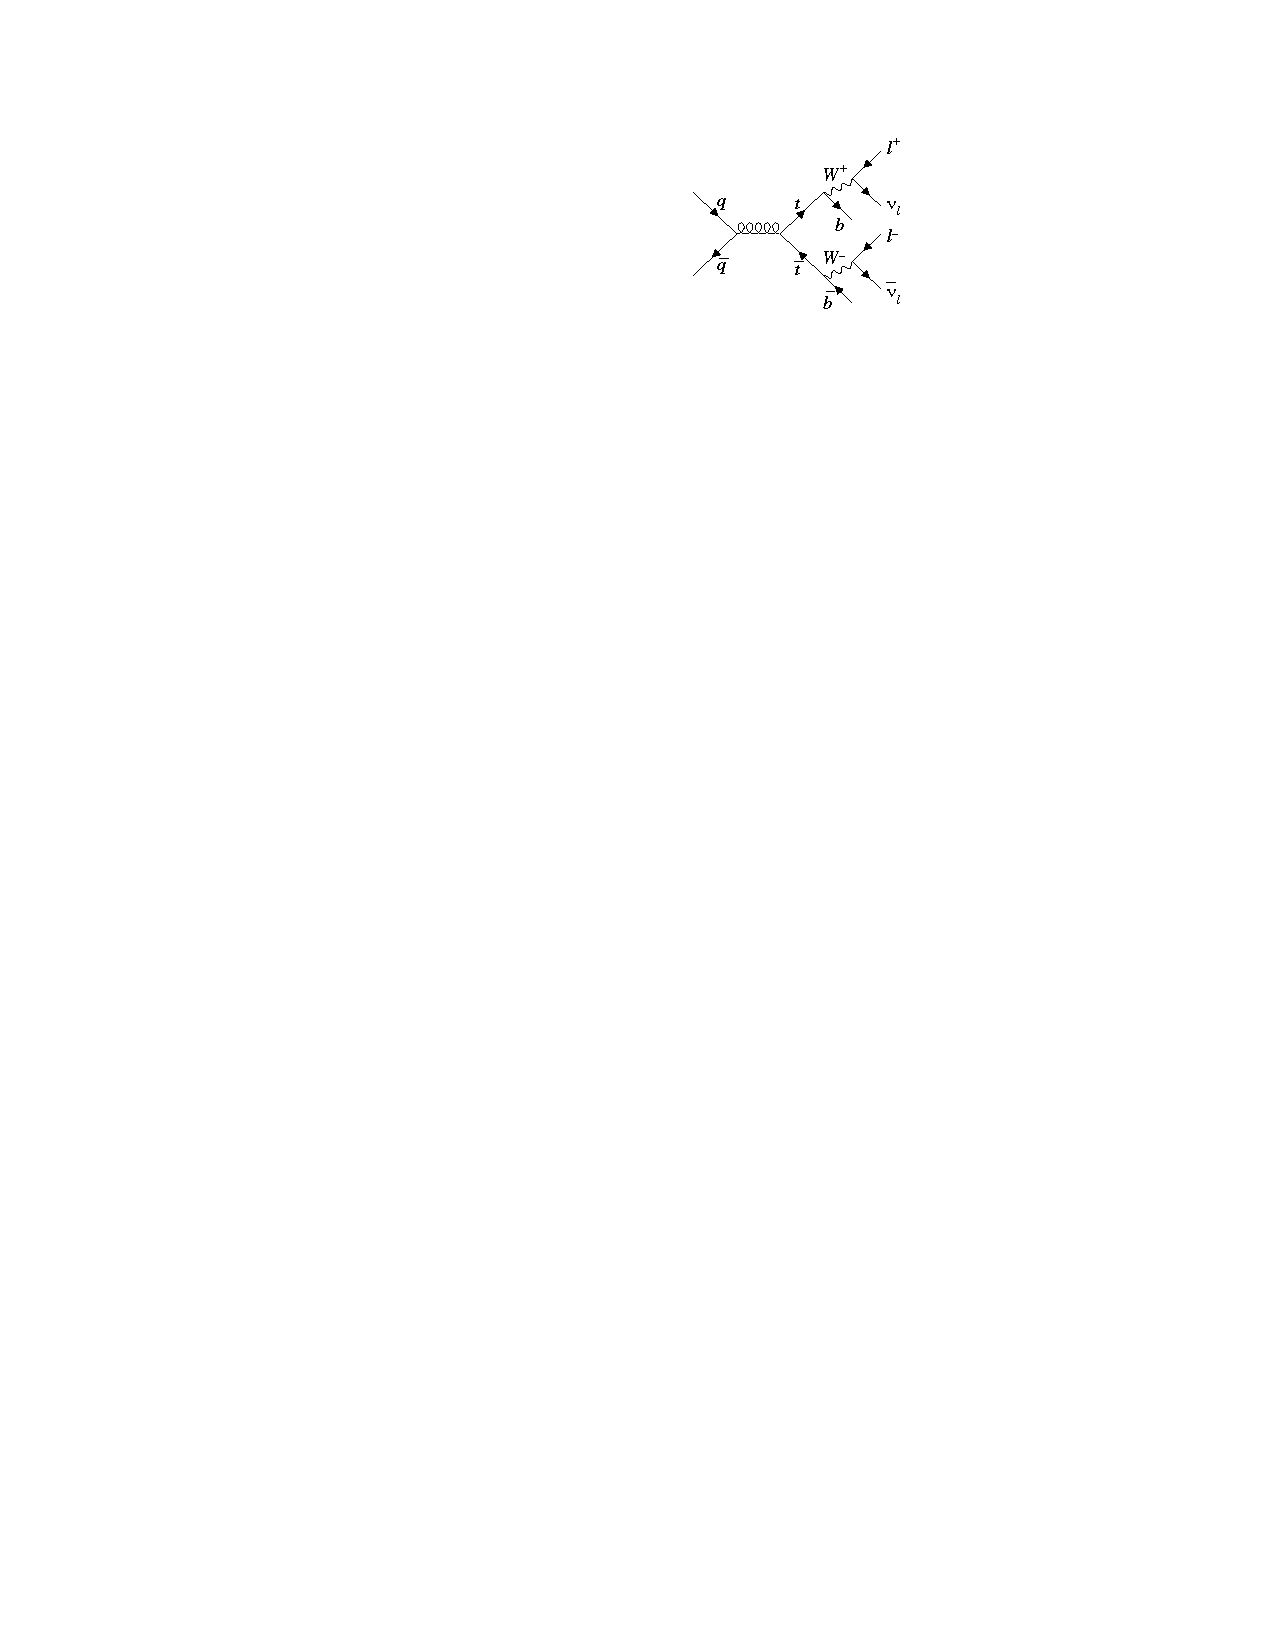
\includegraphics[width=0.7\linewidth, angle=0]{figs/Theory/ttbar.pdf}
  \end{center}
  \caption[A Feynman diagram showing an example of a di-lepton $t\bar{t}$ event.]
  {A Feynman diagram showing an example of a di-lepton $t\bar{t}$ event~\cite{theo-ttbar_feyn}.}
  \label{fig:theo-ttbar}
\end{figure}

Di-lepton $t\bar{t}$ forms a distinct experimental signature.
In particular two leptons of different flavours in an event signifies
that there has likely been two separate weak-decays which would typically be suppressed,
but here the large mass of the top overcomes this suppression.
In addition we have two jets formed from $b$-quarks, which can be observed.
The distinct signature of di-lepton $t\bar{t}$ events and the fact that they always contain $b$-jets
means that this decay topology is often used to obtain a pure sample of $b$-jets, such as in Section~\ref{sec:obj-bjets_calib}~and~\ref{sec:trig-bjet_eff}. 

\clearpage
\section{Beyond the Standard Model}
\label{sec:theo-bsm}

The preceeding sections of this chapter described the Standard Model
and some of its sucesses,
such as the prediction of a Higgs Boson and the ability to describe complex phenomena such as di-jet production.

However, the Standard Model is known to be an incomplete picture of the universe;
in this section I will discuss some of the key deficiencies of the Standard Model as it stands
and why Beyond Standard Model (BSM) physics is required.
I will then discuss some models and search philosophies which may help us progress towards a new underlying theory of Particle Physics.

\subsection{Motivations for Beyond the Standard Model}

The motivations for BSM physics listed in this section
describe only a subset of deficiencies of the Standard Model,
with a focus on the most important missing parts and
those that motivate models searched for in this thesis.

\subsubsection{Gravity}

When listing forces in Section~\ref{sec:theo-sm_forces}, we made no reference to gravity.
This is because our description of gravity, Einstein's General Theory of Relativity,
has not been succesfully merged with Quantum Physics in a so-called `Quantum Theory of Gravity'.
It is a clear inadequecy of the Standard Model that there is no explanation of gravity
%partly due to the fact that gravity is hard to study at the quantum-level because
%it is so much weaker than the other forces
%(of order $10^{-39}$ compared to the strong interaction) .
% \textbf{LM Fix: Reference?}.
%There have been theoretical attempts to decribe gravity such that it is comptible with the Standard Model,
%such as the Randall-Sundrum Graviton~\cite{theo-bsm_randall},
%but so far these have not been substantiated by experimental evidence.%~\cite{trig-H4b}.

\subsubsection{Dark Matter}
\label{sec:theo_bsm_dm}

%It is remarkable that the physics that describes the largest and smallest scale known,
%Astronomy and Particle Physics,
%are often deeply related; the prediction of Dark Matter (DM) is a great example of this.

%Astronomers are able to make observations of distant galaxies using
%EM-waves, that allows observation of Standard Model particles  
%and are have been succesful in explaining the observed galaxies in terms of the particles of the Standard Model,
%listed in Section~\ref{sec:theo-sm_particles}.
%However, due to the large masses of astronomical objects,
%astronomers also have access to observing the action of gravity.

Astronomers are able to make observations of distant galaxies and stars
to study their dynamics in terms of both Standard Model proccesses
and, due to the large masses of galaxies, gravitional interactions.
This has meant that astrophysicists have made a remarkable observation that
80\% of the universe's matter must be so-called `Dark Matter'~\cite{theo-bsm_dm_peskin}.
Dark Matter are particles not described by the Standard Model,
so is clear evidence of Beyond Standard Model physics.
It is known that Dark Matter must interact weakly with the Standard Model,
otherwise we would have already observed it through interactions with Standard Model particles,
and that Dark Matter must be massive, otherwise it would not interact through gravity.

The evidence for Dark Matter comes from many seperate astronomical observations:
such as studies of
gravitational rotation curves,
colliding galaxies known as bullet clusters,
and the cosmic microwave background.
%and galaxies using gravitataional lensing.
A wider summary of the evidence for Dark Matter can be found here~\cite{theo-bsm_dm_evidence}

\begin{figure}[!b]
  \begin{center}
    \captionsetup[subfigure]{aboveskip=0pt,justification=centering}
    \subcaptionbox{Visible Spectrum}{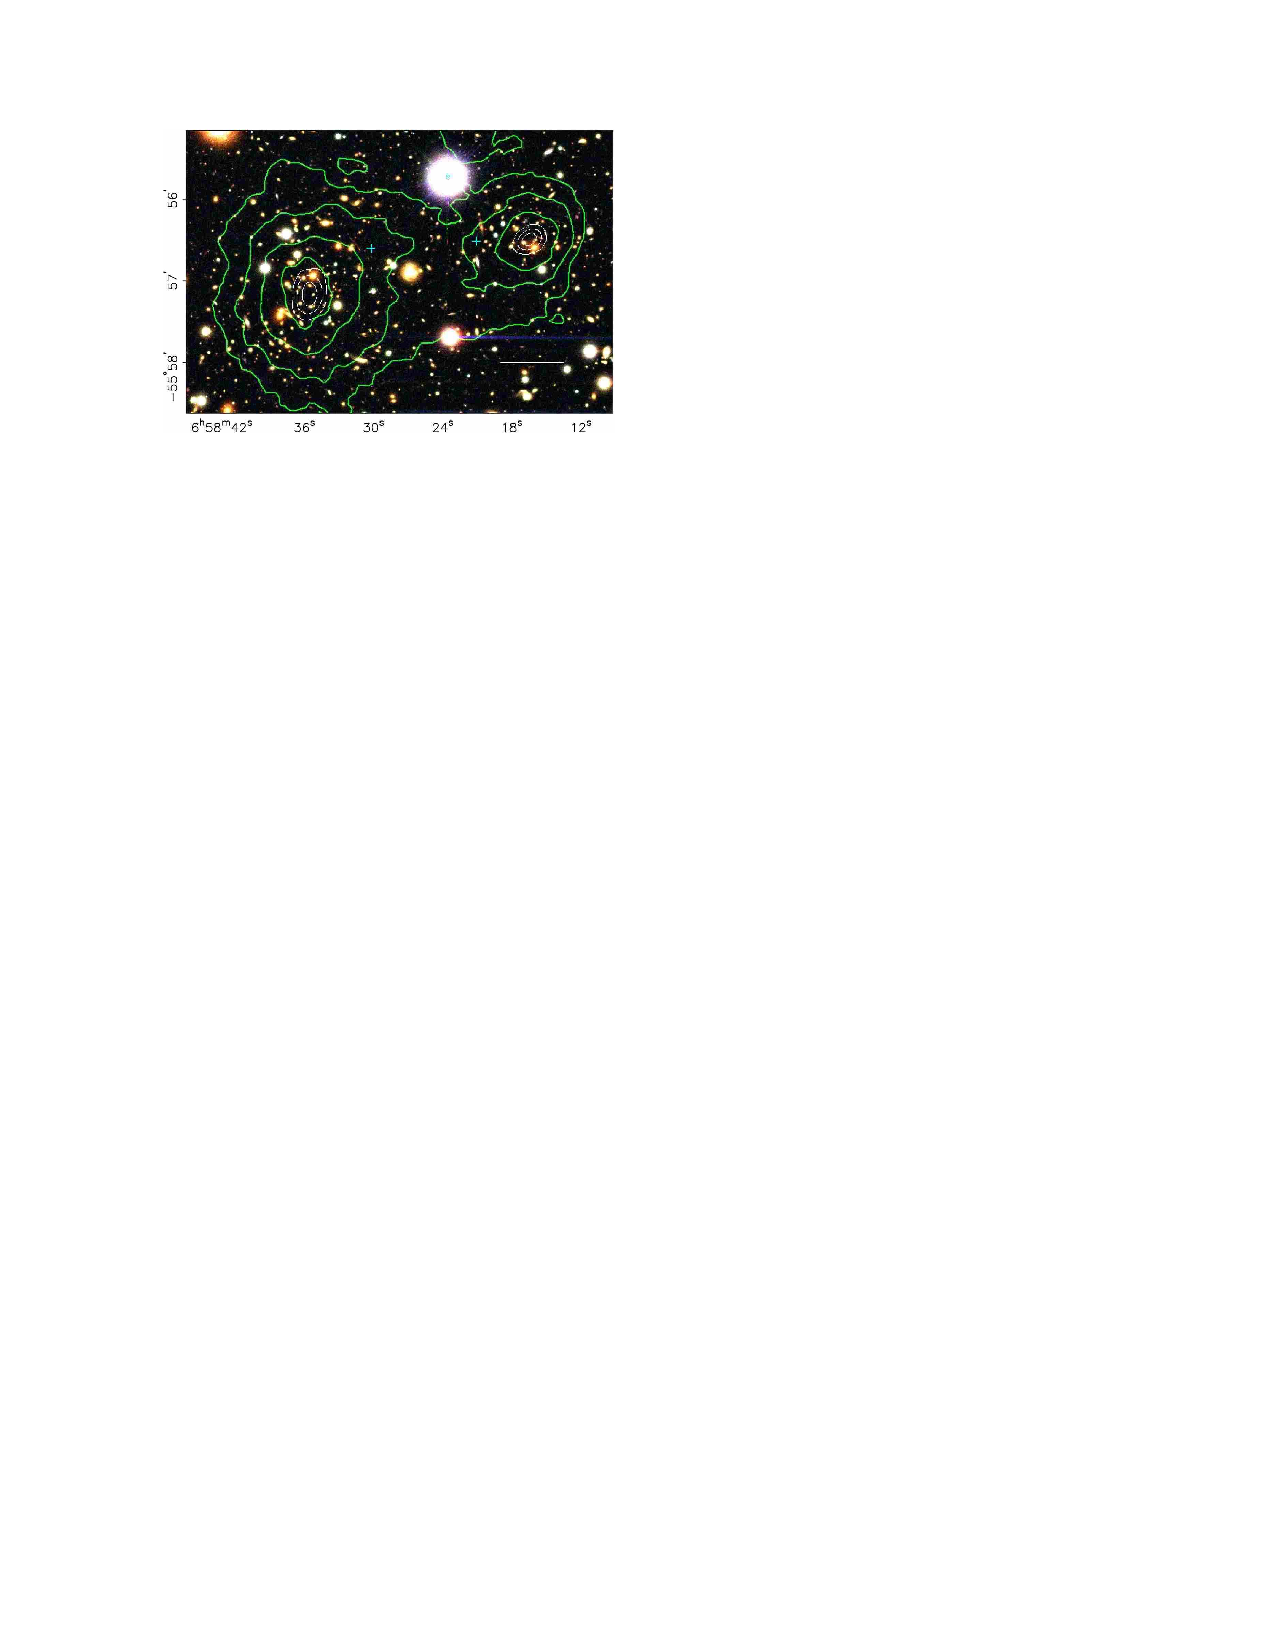
\includegraphics[width=0.48\linewidth, angle=0]{figs/Theory/bsm_gl_vis} }
    \subcaptionbox{X-Ray Spectrun}{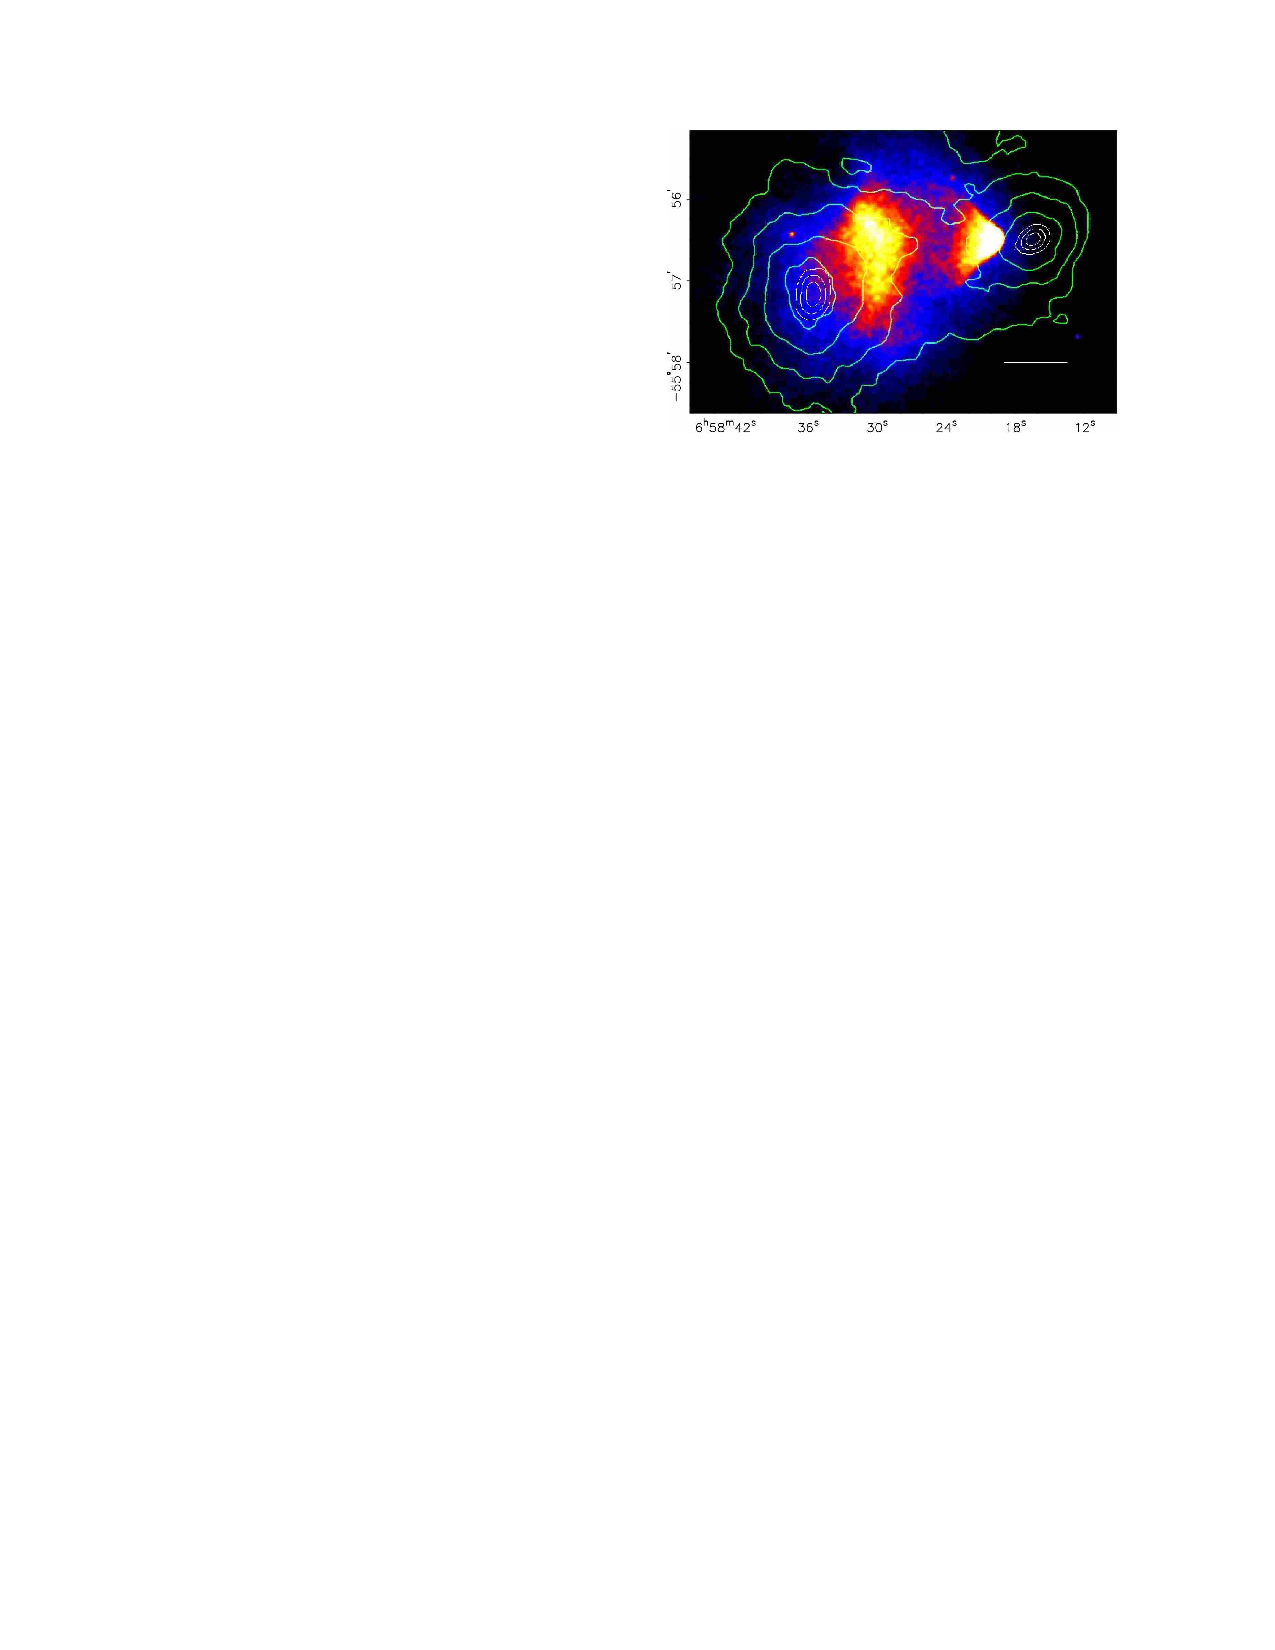
\includegraphics[width=0.48\linewidth, angle=0]{figs/Theory/bsm_gl_xray}}
  \end{center}
  \caption{An image of the same bullet cluster
    (a) in the visible spectrum using the Hubble Space Telescope
    and (b) in the X-ray spectrum using the Chandra telescope.
    The mass density profile estimated using gravitiational lensing is overlaid on both plots.}
  \label{fig:theo-bsm_dm_gl}
\end{figure}

The cited summary provides a more rigorous explanation of the evidence than can be provided here.
But I would like to discuss one particular bit of evidence,
specifically measurements of bullet clusters using X-ray telescopes and gravitational lensing~\cite{theo-bsm_dm_gl}.
Gravitational lensing occurs when the path of light from some distant astronomical source is bent by the gravitational effect of a nearer galaxy.
Figure~\ref{fig:theo-bsm_dm_gl}(a) shows an image of a bullet cluster and the surrounding galaxies in the visible part of the light spectrum using the Hubble telescope.
Using the gravitiational lensing effect in this image one can infer the mass density profile of the bullet cluster, which is shown by the green contour lines.
One can also observe the galaxy using an X-ray telescope,
allowing an observation of the number density profile of Standard Model particles in a galaxy which, when hot, will emmit X-ray radiation.
Figure~\ref{fig:theo-bsm_dm_gl}(b) shows an image of the same bullet cluster in the X-ray part of the light spectrum using the Chandra telescope;
the mass density profile estimated using the visible spectrum has again been overlaid.
One can see that the mass density profile of the bullet cluster is inconistent with the
number density profile of the Standard Model particles from the X-ray telescope.
Hence one can conclude that there must be additional Dark Matter particles in this bullet cluster
causing the shift in the mass density profile.

Furthermore it is believed that the Dark Matter couples to the Standard Model;
the evidence for such a statment stems from the observed abundance of Dark Matter particles in the universe.
The most common method of explaining the abundance
%, known as 'freeze-out',
argues that in the early and hot universe Dark Matter and Standard Model particles
freely interact such that they are in thermal equilibrium.
As the universe expands and cools this interaction is supressed
and the number density of Dark Matter is fixed at the value we observe today~\cite{theo-bsm_dm_feng}.
%The most common method of explaining the abundance is by postulating that
%DM and SM particles were produced in the same abundance in the Big Bang,
%and in the early hot and dense universe they could interact freely such that they are in thermal equilibrium.
%As the universe begins to cool and expand this number density will fall in equilibrium with the SM particles.
%However, at some point the universe is sufficiently cool that this interaction becomes supressed and the
%number density of Dark Matter is fixed at the value we observe today; this process is known as 'freeze-out'.
As a result this means that there may be some yet unkown mechanism that couples to both Dark Matter and
Standard Model particles; this mechanism is referred to as a Dark Matter mediator
something which one can search for at the LHC experiment.
%%%%% Note to laurie
%% => WIMP is if mediator is weak and particle is massive
%% => WIMP miracle is that freeze-out occurs at roughly right abundance with no extra work. Great news
%% => Unfortunately WIMP is starting to become very constrained (https://arxiv.org/pdf/1507.03800.pdf)
%% => So we might need other mediator models, such as the Z'.
\textbf{Do I need to talk about the WIMP miracle; I was going to say no as I want to talk about Z' which is not the weak force as such}

\subsubsection{Hierachy Problem}

The Hierachy problem is the fact that the mass scale of electro-weak breaking, ($M_{EW}\nobreak\sim\nobreak100~\text{GeV}$),
is much smaller than the mass scale of gravity,
known as the Plank scale ($M_{Plank}\nobreak\sim\nobreak10^{19}~\text{GeV}$).
This effecitvely means that the energy scale of the physics we see in the Standard Model is very far
from the energy scale of the next known interaction, that of gravity.

The Hierachy problem leads to complications in theoretical calculations, such as the that of the Higgs Boson mass.
When calculating the Higgs Boson mass one must consider the bare mass of the Higgs Boson from the Lagrangian
in addition to radiative contributions from additional loop diagrams,
similar to what was done for the gluon propagator in Section~\ref{sec:theo-qcd_dijet_running}.
However, when one performs the calculation for these additional loops, there is a divergent integral
such that contributions are found to be of the order $\delta m_H^2 \sim \frac{1}{16\pi^2} M_{Plank}^2$.
These contributions are much larger than the observed mass of the Higgs boson,
meaning that in reality some mechanism must cancel the contributions or reduce their size.
Whilst the parameters from the Standard Model can be chosen such that these different contribtutions approximately cancel out,
such fine-tuning of the parameters of the Standard Model theory is hard to believe without some underlying explanation.

Instead there are two solutions typically proposed to reduce the effect of the loop corrections.
Firstly, one can introduce BSM physics through a new symmetry such that Standard Model contributions are cancelled by the BSM contributions.
Secondly, one can introduce some BSM physics,
such that the divergent integral can have a new cut-off scale,
and the loop diagram contributions become $\delta m_H^2 \sim \frac{1}{16\pi^2} M_{BSM}^2$.
If the BSM physics is on the TeV scale then this would lead to corrections of the scale of the Higgs boson.
Both solutions suggest that there might be BSM physics around the TeV scale, possibly within the energy reach of the LHC experiment

\subsubsection{Quarks Generational Structure}
\label{sec:theo-bsm_3g}

The quarks of the standard model have a well ordered generational symmetry,
three generations of quarks that are in a pair of $+\frac{2}{3}$ and $-\frac{1}{3}$ quarks.
However the generational symmetry is not perfect;
each generation is heavier than the previous one
and within the generations quarks can have different masses.
In particular, the third generation of quarks is somewhat special;
the top quark is much heavier than the bottom quark
and is the heaviest particle of the Standard Model.

There is no good explanation of why there is generational structure in the Standard Model,
why the structure is unsymmetric 
or why the third generation has one quark with such a large mass.
The generational structure could be a result of some underlying broken symmetry
which forms a part of a deeper theory of Particle Physics.
Any deeper theory explanaing the generational structure could contain observable BSM particles,
and, given the special nature of the third generation,
the BSM particles could couple strongest with the third generation of quarks.

Unlike the case of Dark Matter,
the generational structure of quarks
and the special nature of the third generation is not concrete evidence
of BSM physics.
But it does mean that there are some reasons to be particularly interested in the
searches for particles decaying to the third generation of quarks.

\newpage
\subsection{Beyond Standard Model Theories}

The previous section discussed a list of deficiencies of the Standard Model,
which makes us confident that there must be a theory of physics Beyond the Standard Model.
Many theories of BSM physics include the addition of a new particle,
which one can test by searching for the production of such a particle in a particle collider experiment.

In particular, the special nature of the third generation
\footnote{Discusssed in Section~\ref{sec:theo-bsm_3g}}
means that some models of BSM predict new particles
that decay to one or two $b$-quarks
with an enhanced branching ratio.
Further to this the Hierachy Problem gave us some motivation
that any new physics may be at the TeV scale,
which means that we can search for this at the energy range of the LHC.

Below two such models that predict resonances at the TeV scale with preferential decays to $b$-quarks
are discussed.
These are used as `benchmark models' in the analysis presented in this thesis,
where a benchmark model is a plausible signal model 
that is used to form and optimise a search strategy.

\subsubsection{$Z'$ Boson}

One of the most simple additions to the Standard model is that of a $U(1)'$ gauge symmetry
which would result in an additional $Z'$ boson.
The $Z'$ model can decay to a pair of $b$-quarks, as shown in Figure~\ref{fig:theo_bsm_zprime}.
An additonal $U(1)'$ symmetry appears in many different BSM models and is therefore a well motivated BSM extension~\cite{theo-bsm_zprime}.
%Often theses models use the breaking of some higher gauge symmetry to give $G_{SM}~\text{x}~U'(1)^n$ gauge symmetry group,
%and thus giving additional predicting the existence of new gauge bosons in addition to the Standard Model
%\footnote{$G_{SM} = SU(3)~\text{x}~SU(2)~\text{x}~U(1)$, which is the gauge symmetry group of the Standard Model discussed in Section~\ref{sec:theo-sm}}.

In this thesis we will consider three different models of $Z'$ boson.
The first is known as the Sequential Standard Model (SSM) $Z'$ in which the couplings
of the new $Z'$ boson are set to match those of the Standard Model, leading to universal coupling to all fermions.
The strongest limits on the SSM $Z'$ boson at the TeV scale are set by searching for $Z'$ decaying to lepton pairs~\cite{theo-bsm_dilep},
due to the fact that this signature is distinct to the large QCD dijet backgrounds produced in $pp$ collisions.
In addition, we also consider a leptophobic $Z'$ model that does not couple to the lepton sector
but has equal coupling to the quark sector~\cite{theo-bsm_zprime_leptophobic},
this model is therefore not strongly constrained by di-lepton searches.

The final $Z'$ model considered acts as a Dark Matter mediator which can couple to both the Dark Matter sector and the Standard Model quark sector~\cite{theo_bsm-zprime_dm};
the motivation for such a model was discussed in Section~\ref{sec:theo_bsm_dm}.
This model introduces an additional $U(1)'$ symmetry and a Dirac fermion Dark Matter particle that only interacts through the new gauge group.
The resulting $Z'$ couples to the DM fermion with a coupling $g_\chi$\vspace{0.1mm},
couples to the Standard Model quark sector with a coupling $g_q$\vspace{0.1mm},
and is leptophobic such that it does not couple to the lepton sector.

It is worth noting that the $Z'$ models considered do not preferentially decay to 3rd generation quarks but rather with equal branching ratio.
This is still advantageous as the dominant dijet background produces jets preferentially
initiated by gluons or quarks from the first two generations, as discussed in Section~\ref{sec:theo-qcd_dijet}.
Furthermore there exist $Z'$ models not considered here that predict couplings to fermions that are not equal amongst all generations~\cite{theo-bsm_3g}
which the analyses presented in this thesis are sensitive to.

%For example; attempts to merge the electro-weak and strong interactions in a so-called 'Grand Unified Theory'
%often use higher symmetries, such as $SU(5)$ or $SO(10)$.

\subsubsection{Excited Third-Generation Quark}

To explain the generational and mass structure of the quark sector, discussed in Section~\ref{theo-bsm_3g},
quark compositeness models describe quarks, not as fundamental particles, but instead constructed of other fundamental particles.
One concequence of quark compositeness models is the prediction of excited quarks, $q^{*}$, which can be observed as heavy resonances.
In particular we consider an excited 3rd generation quark, the $b^{*}$ quark, which has a dominant decay to a $b$-quark and a gluon
as shown in Figure~\ref{fig:theo_bsm_bstar}.

The exact branching ratios (BRs) of the excited quark's decay are results of features of the quark compositeness model.
In this thesis we consider a naive  excited quark model where the scale of the effective Lagrangian is set to the excited-quark mass,
as described in~\cite{theo-bsm_bstar}.
In this model the dominant decay mode is to $bg$ with a BR of 85\%
while the remaining decay modes are to $Wt$, $bZ$ and $b\gamma$ with BRs of 10\%, 4.5\% and 0.5\% respectively. 

\subsubsection{Model Independance}

The two benchmark models indicate that searching for particles decaying to one or two $b$-quarks.
However, it is important to note the prior expectation in any specific model of BSM is quite low.
This is because there are many BSM theories that exist
which could explain some of the problems explained in the previous section and
there is little direct or indirect evidence to prefer one model over another.
In addition, one must also consider that the true theory may yet to be realised
so experimentalists might see evidence of some signature of something unexpected.

Therefore, one should construct searches for BSM to be as model independant as possible,
rather than optimising specifically for any one model in particular.
In our case we want to search for any particle that is decaying to one or two
$b$-quarks, in a way such we include as any BSM theoretical models as possible
and allow for the unexpected gifts that nature might throw up.
